\begin{problem}{F: Checkmate In One}

There are several different types of pieces in chess. We're going to focus on three for this problem: kings, queens, and knights. Below is a description of each piece for those who need a review of the rules. Recall that chess is played on an 8x8 board with pieces that are two colors, typically black and white.

The king is the most important piece in the game. Its move and attack pattern can be seen belown. It can move/attack any square that's next to it. Unlike the other pieces, it cannot be captured. It can, however, be attacked (this is called being in check). It's illegal to make any move that puts your own king in check. If the king is in check, the player's next move must be to move out of check. If this is not possible, the player loses (this is called checkmate).

\begin{figure}[h]
    \centering
    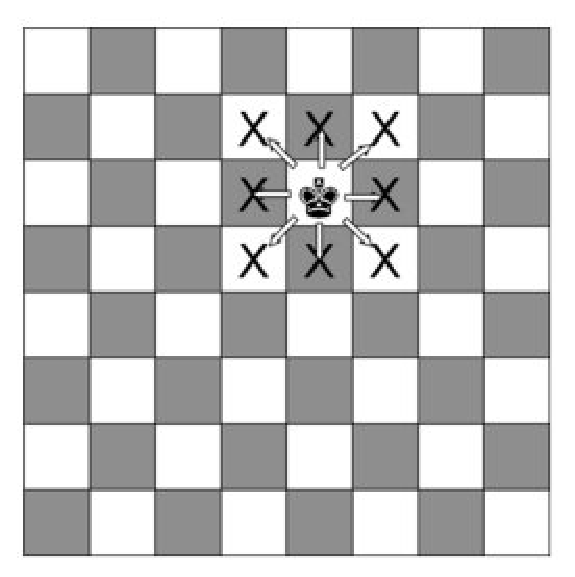
\includegraphics[width=0.2\textwidth]{king-moves.eps}
\end{figure}

Queens are the most powerful piece in the game. Its move/attack pattern can be seen below. They can move as many spaces they want in any single direction, unless there is a piece blocking their way. That is, queens cannot move or attack through other pieces.

\begin{figure}[h]
    \centering
    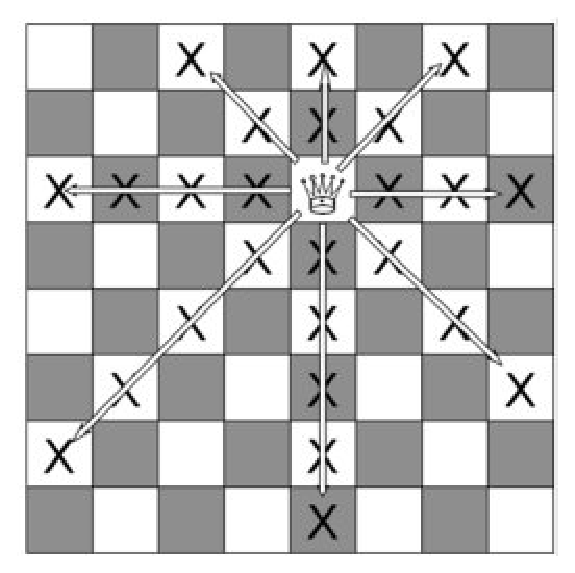
\includegraphics[width=0.2\textwidth]{queen-moves.eps}
\end{figure}

Knights are the only piece that can jump over other pieces. They move/attack in an L-shape, jumping over any pieces it takes to reach that square. They move two spaces in one direction and one space in another.

\begin{figure}[h]
    \centering
    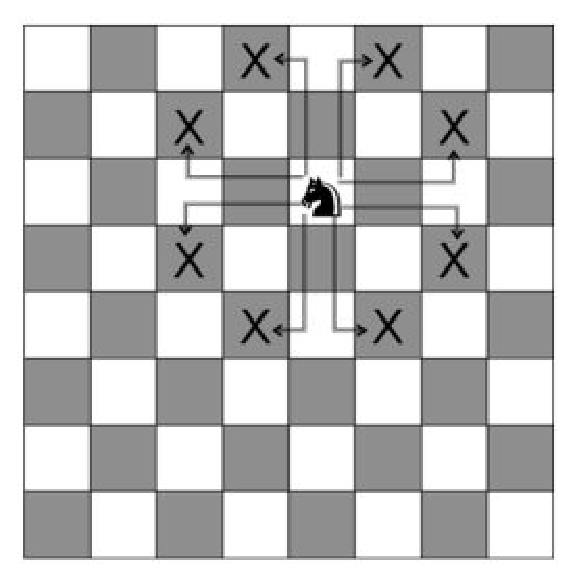
\includegraphics[width=0.2\textwidth]{knight-moves.eps}
\end{figure}

When a piece is captured, the piece is removed from the board and the attacking piece moves to that location. Pieces can only capture pieces of the opposite color. Under no circumstance can a king be captured. A piece cannot be moved if doing so puts their own king in check.

In our problem, you play as white, an arrogant snob who's wiping the floor with your opponent. Black only has a single piece left: their king. It's your turn. Black is determined to drag out the game forever, but you've got a hot date later and you don't want to miss it for chess. Again. So your goal is to write a program that answers this simple question: is it possible to checkmate black after a single move?

\end{problem}

\begin{formalin}
Input consists of eight lines, describing the board and pieces on it. Each lines consists of eight characters representing the pieces, and seven spaces separating them. White's king, queens, and knights are respresented by the characters 'K', 'Q', and 'N' respectively. Black's king is represented as '\$', and an empty space is represented as '.'. It is guaranteed that there is exactly one white king and one black king on the board.
\end{formalin}

\begin{formalout}
Output "yes" if you can checkmate black in one move, or "no" otherwise.
\end{formalout}


\begin{datain}
. . . . . . . Q
. Q . . . . . .
. . . . . . . .
. . . . . . . .
. . . . . . . .
. . . . . . . .
. . . . . . . .
$ . . . . . . K
\end{datain}
\begin{dataout}
yes
\end{dataout}

\begin{datain}
N . . . . . . N
. . . . . . . .
. . . . . . . .
. . . . $ . K .
. . . . . . . .
. . N . . . . .
. . . . . . . .
Q . . . . . . N
\end{datain}
\begin{dataout}
no
\end{dataout}

\begin{datain}
K . . . . . . .
. . . . N . . .
Q . . . . . . .
. . $ . . . . .
Q . . . . . . .
. . . . . . . .
. . . . . . . .
. . N . . . . .
\end{datain}
\begin{dataout}
yes
\end{dataout}

